\chapter{\chapFont 耶稣的降生}
\setmark{耶稣的降生}

2018年1月21日 \hfill 路加福音第2章

\BibSentence{腓}{2}{6-7}{他本有神的形像,不以自己与神同等为强夺的。反倒虚己,取了奴仆的形像,成为人的样式。}

\section{查考的背景资料}

\begin{enumerate}
  \item \textbf{基督降生的背景}: 被虏的犹太人,盼望神应许的弥赛亚(救世主)的到来,拯救他们脱离困境,重归应许之地。\\
  \BibT{赛}{9}\BibS{6}{因有一婴孩为我们而生,有一子赐给我们。政权必担在他的肩头上。他名称为奇妙,策士,全能的神,永在的父,和平的君。}\BibS{7}{他的政权与平安必加增无穷。他必在大卫的宝座上,治理他的国,以公平公义使国坚定稳固,从今直到永远。万军之耶和华的热心,必成就这事。}
  \item \textbf{作者路加}:保罗传道时的同工,《路加福音》《使徒行传》的作者。《圣经》只提到他三次。根据保罗书信中透露的信息可以得知,路加的职业是医生,使徒保罗称他为“亲爱的医生”和“我的同工”\cite{wiki:Luke}。
  \item \textbf{《路加福音》写作的背景}:保罗被关押,路加写这本福音书给提阿非罗大人,为教会和保罗辩护。
\end{enumerate}

\section{正文预查}

\begin{Parallel}[v]{\BibLength}{\TexLength}
  \litem{\BibT{路}{1}\BibS{26}{到了第六个月,天使加百列奉{\Lord}的差遣,往加利利的一座城去,这城名叫拿撒勒。}}
  \ritem{}
  \litem{\BibS{27}{到一个童女那里,是已经许配大卫家的一个人,名叫约瑟,童女的名字叫马利亚。}}
  \ritem{旧约预言了基督由童女所生:\BibT{赛}{7}\BibS{14}{因此,主自己要给你们一个兆头,必有童女怀孕生子,给他起名叫以马内利。(就是{\Lord}与我们同在的意思)}}
  \litem{\BibS{28}{天使进去,对她说,蒙大恩的女子,我问你安,主和你同在了。}}
  \ritem{}
  \litem{\BibS{29}{马利亚因这话就很惊慌,又反复思想这样问安是什么意思。}}
  \ritem{这是马利亚第一次“反复思想”。这里马利亚可能在思想什么?(可能是在惊诧于自己蒙的恩是什么。)}
  \litem{\BibS{30}{天使对她说,马利亚不要怕。你在{\Lord}面前已经蒙恩了。}}
  \ritem{}
  \litem{\BibS{31}{你要怀孕生子,可以给他起名叫耶稣。}}
  \ritem{这是来自于神的恩典和智慧,神已经启示,要藉着主耶稣拯救百姓。\BibT{太}{1}\BibS{21}{她将要生一个儿子。你要给他起名叫耶稣。因他要将自己的百姓从罪恶里救出来。}}
  \litem{\BibS{32}{他要为大,称为至高者的儿子。主{\Lord}要把他祖大卫的位给他。}}
  \ritem{神早已应许大卫,要坚立他的国到永远。因此差下耶稣基督,作大卫的后裔。\BibT{撒下}{7}\BibS{12}{你寿数满足,与你列祖同睡的时候,我必使你的后裔接续你的位。我也必坚定他的国。}}
  \litem{\BibS{33}{他要作雅各家的王,直到永远。他的国也没有穷尽。}}
  \ritem{\BibT{撒下}{7}\BibS{16}{你的家和你的国必在我(原文作你)面前永远坚立。你的国位也必坚定,直到永远。}}
  \litem{\BibS{34}{马利亚对天使说,我没有出嫁,怎么有这事呢?}}
  \ritem{显示了童女生子的异乎寻常。在古代,未婚先孕又要证明贞节是非常难的,马利亚可能要为此背负不名誉和受到指责的危险。}
  \litem{\BibS{35}{天使回答说,圣灵要临到你身上,至高者的能力要荫庇你。因此所要生的圣者,必称为{\Lord}的儿子。(或作所要生的必称为圣称为{\Lord}的儿子)}}
  \ritem{}
  \litem{\BibS{36}{况且你的亲戚以利沙伯,在年老的时候,也怀了男胎。就是那素来称为不生育的,现在有孕六个月了。}}
  \ritem{}
  \litem{\BibS{37}{因为出于{\Lord}的话,没有一句不带能力的。}}
  \ritem{}
  \litem{\BibS{38}{马利亚说,我是主的使女,情愿照你的话成就在我身上。天使就离开她去了。}}
  \ritem{显示了马利亚的信心。我们要学习马利亚。}
  \litem{\BibT{路}{2}\BibS{1}{当那些日子,该撒亚古士督有旨意下来,叫天下人民都报名上册。}}
  \ritem{}
  \litem{\BibS{2}{这是居里扭作叙利亚巡抚的时候,头一次行报名上册的事。}}
  \ritem{}
  \litem{\BibS{3}{众人各归各城,报名上册。}}
  \ritem{}
  \litem{\BibS{4}{约瑟也从加利利的拿撒勒城上犹太去,到了大卫的城,名叫伯利恒,因他本是大卫一族一家的人。}}
  \ritem{因着报名上册的事,成就了神的预言。很多这样不经意的事,恰恰体现了神奇妙的作为。\BibT{弥}{5}\BibS{2}{伯利恒,以法他阿,你在犹大诸城中为小。将来必有一位从你那里出来,在以色列中为我作掌权的。他的根源从亘古,从太初就有。}}
  \litem{\BibS{5}{要和他所聘之妻马利亚,一同报名上册。那时马利亚的身孕已经重了。}}
  \ritem{}
  \litem{\BibS{6}{他们在那里的时候,马利亚的产期到了。}}
  \ritem{}
  \litem{\BibS{7}{就生了头胎的儿子,用布包起来,放在马槽里,因为客店里没有地方。}}
  \ritem{
      1. 须知主降生在马槽,是祂自己的选择。在未来,主也这样一次次地选择尝过人世的种种痛苦和试探,所以祂能体察、体谅我们生而为人的艰难。\BibT{来}{2}\BibS{18}{他自己既然被试探而受苦,就能搭救被试探的人。}
      
      2. 试问我们自己,假如我们能选择自己的出生地,我们会做出怎样的选择呢?你觉得耶稣降生应该是什么样子的?(充满光明、亮堂的。)
      
      3. 重点查考主降生和那些伟人降生的不同。例如刘邦、亚历山大,他们也宣称自己是神的儿子,但和主耶稣的降生有本质的不同。
      
      4. 耶稣的选择,表明祂更看重高尚的人格,祂也切身地作出榜样,从一出生就开始奉献自己。一段分享:\textit{当基督来的时候,他藐视一切分别等级的勋章,就是人们籍以表示伟大的东西,却带着地上贫穷和卑微的标记。真的伟大是在品格,绝不是在处境。要确实知道你生命的本质是王族的——虽然你在田间或矿井里劳动,或是在卑下的地方服务,人们却要认出你就是王。他是基督,曾来到地上,接触到人生的最底层,以致他那慈爱和恩典没有人不能得到。}\cite{blog:jeasusManger}
  }
  \litem{\BibS{8}{在伯利恒之野地里有牧羊的人,夜间按着更次看守羊群。}}
  \ritem{为什么要在这里强调牧羊人?《圣经》中“羊”特殊的含义,参见\autoref{fig:cpt1:sheep}。}
  \litem{\BibS{9}{有主的使者站在他们旁边,主的荣光四面照着他们。牧羊的人就甚惧怕。}}
  \ritem{}
  \litem{\BibS{10}{那天使对他们说,不要惧怕,我报给你们大喜的信息,是关乎万民的。}}
  \ritem{关乎万民,也关乎我们每一个人。因为\BibT{约}{14}\BibS{6}{耶稣说,我就是道路,真理,生命。若不借着我,没有人能到父那里去。}}
  \litem{\BibS{11}{因今天在大卫的城里,为你们生了救主,就是主基督。}}
  \ritem{基督就是“受膏者”,只有作王(如大卫)或祭司(如亚伦),才能受膏。基督既是天国永远的王,也是我们每个人的祭司。\BibT{来}{4}\BibS{14}{我们既然有一位已经升入高天尊荣的大祭司,就是神的儿子耶稣,便当持定所承认的道。}}
  \litem{\BibS{12}{你们要看见一个婴孩,包着布,卧在马槽里,那就是记号了。}}
  \ritem{}
  \litem{\BibS{13}{忽然有一大队天兵,同那天使赞美{\Lord}说,}}
  \ritem{}
  \litem{\BibS{14}{在至高之处荣耀归与{\Lord},在地上平安归与他所喜悦的人。(有古卷作喜悦归与人)。}}
  \ritem{从基督降生开始,新的、平安的约就应验到“他所喜悦的人”身上了,这“平安”可以理解为神与人重归于好。}
  \litem{\BibS{15}{众天使离开他们升天去了,牧羊的人彼此说,我们往伯利恒去,看看所成的事,就是主所指示我们的。}}
  \ritem{}
  \litem{\BibS{16}{他们急忙去了,就寻见马利亚和约瑟,又有那婴孩卧在马槽里。}}
  \ritem{}
  \litem{\BibS{17}{既然看见,就把天使论这孩子的话传开了。}}
  \ritem{}
  \litem{\BibS{18}{凡听见的,就诧异牧羊之人对他们所说的话。}}
  \ritem{}
  \litem{\BibS{19}{马利亚却把这一切的事存在心里,反复思想。}}
  \ritem{马利亚的第二次“反复思想”,可见马利亚是个聪明好思的人,她也是个谦卑的人,她领受、感激到自己有福,但是从不夸耀,而是“存在心里”。}
  \litem{\BibS{20}{牧羊的人回去了,因所听见所看见的一切事,正如天使向他们所说的,就归荣耀与{\Lord},赞美他。}}
  \ritem{}
\end{Parallel}

\qquad

\section{其他资料}

\begin{figure}[htbp]
  \centering
  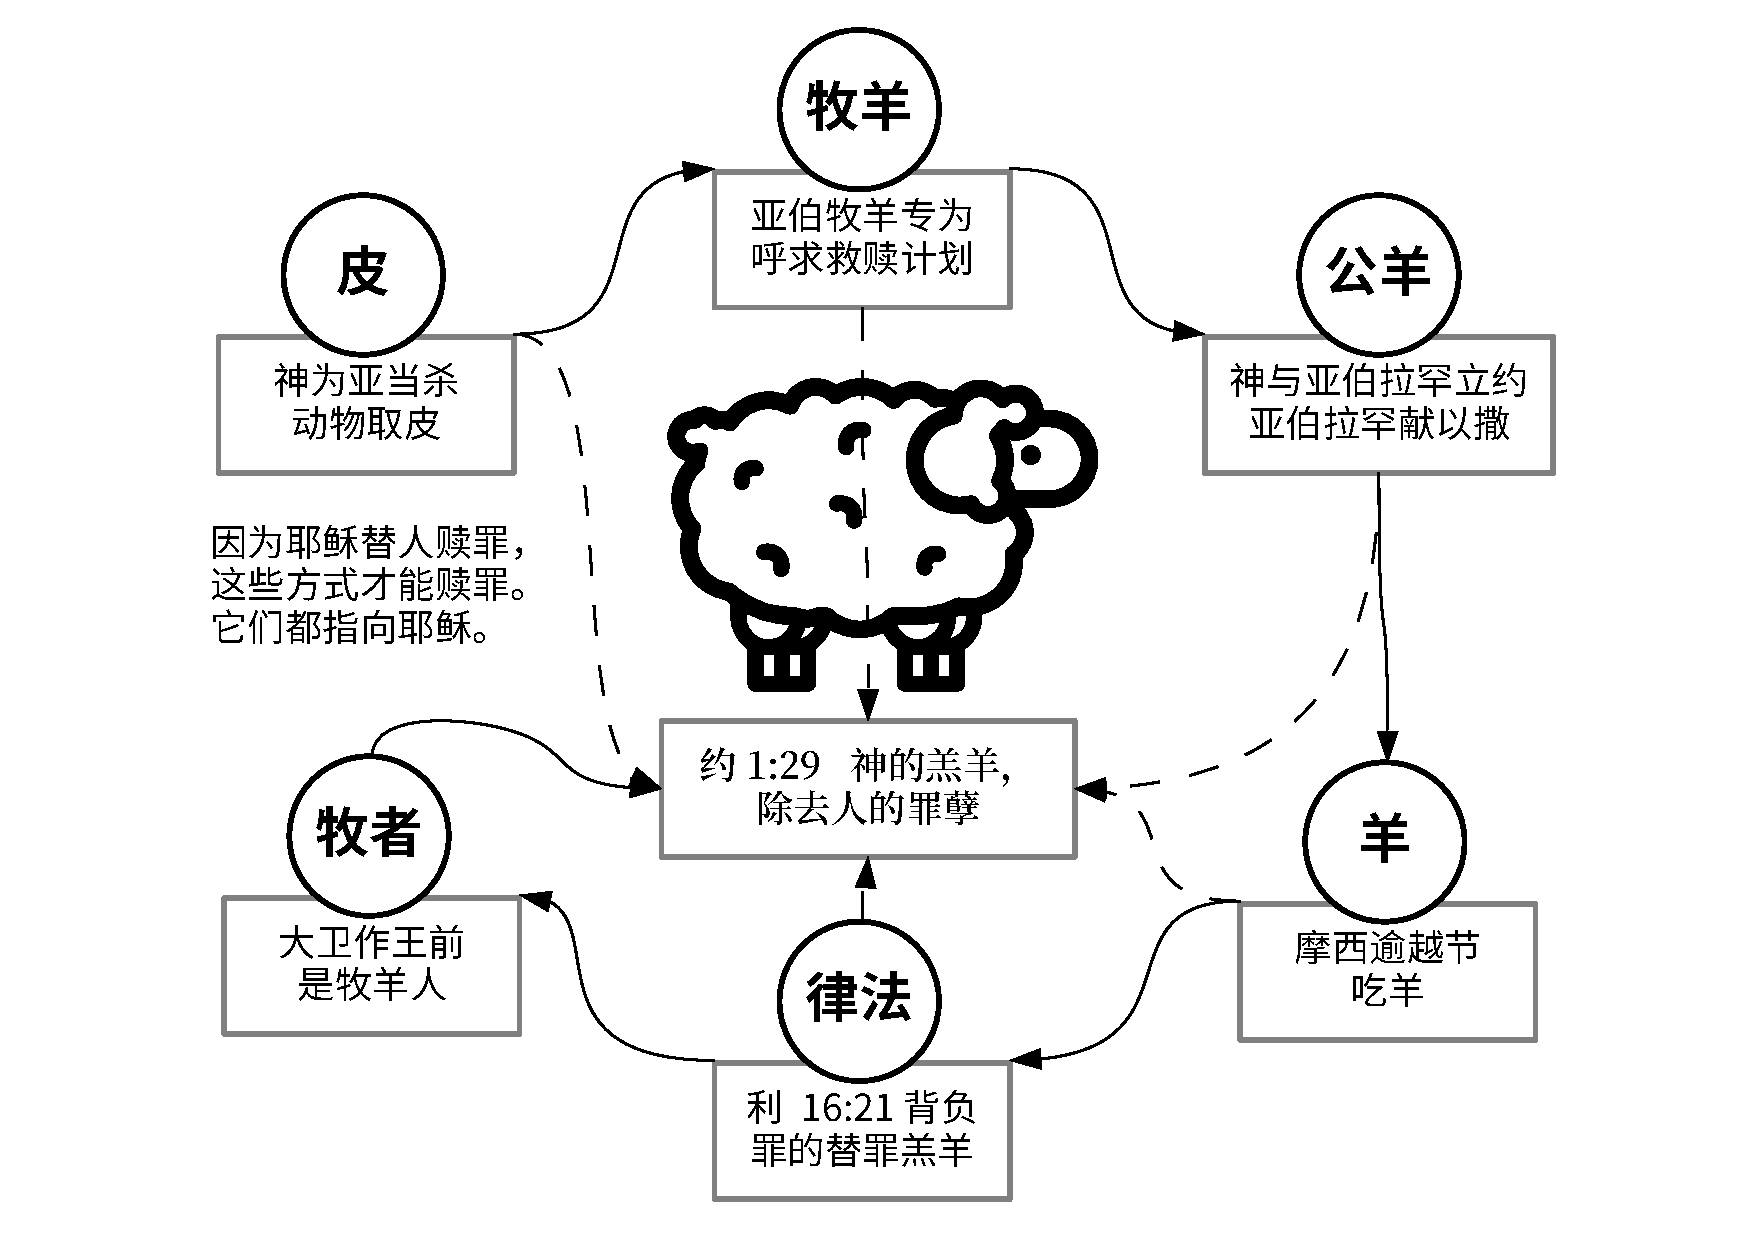
\includegraphics[width = 0.9\textwidth]{tex20180121_sheep.pdf}
  \DeclareGraphicsExtensions.
  \caption{羊的内涵。}
  \label{fig:cpt1:sheep}
\end{figure}

\renewcommand{\bibname}{本章参考}
\bibliographystyle{IEEEtran}
\bibliography{bib/tex20180121}